\documentclass{standalone}
\usepackage{tikz}
\usetikzlibrary{patterns, positioning}


\begin{document}
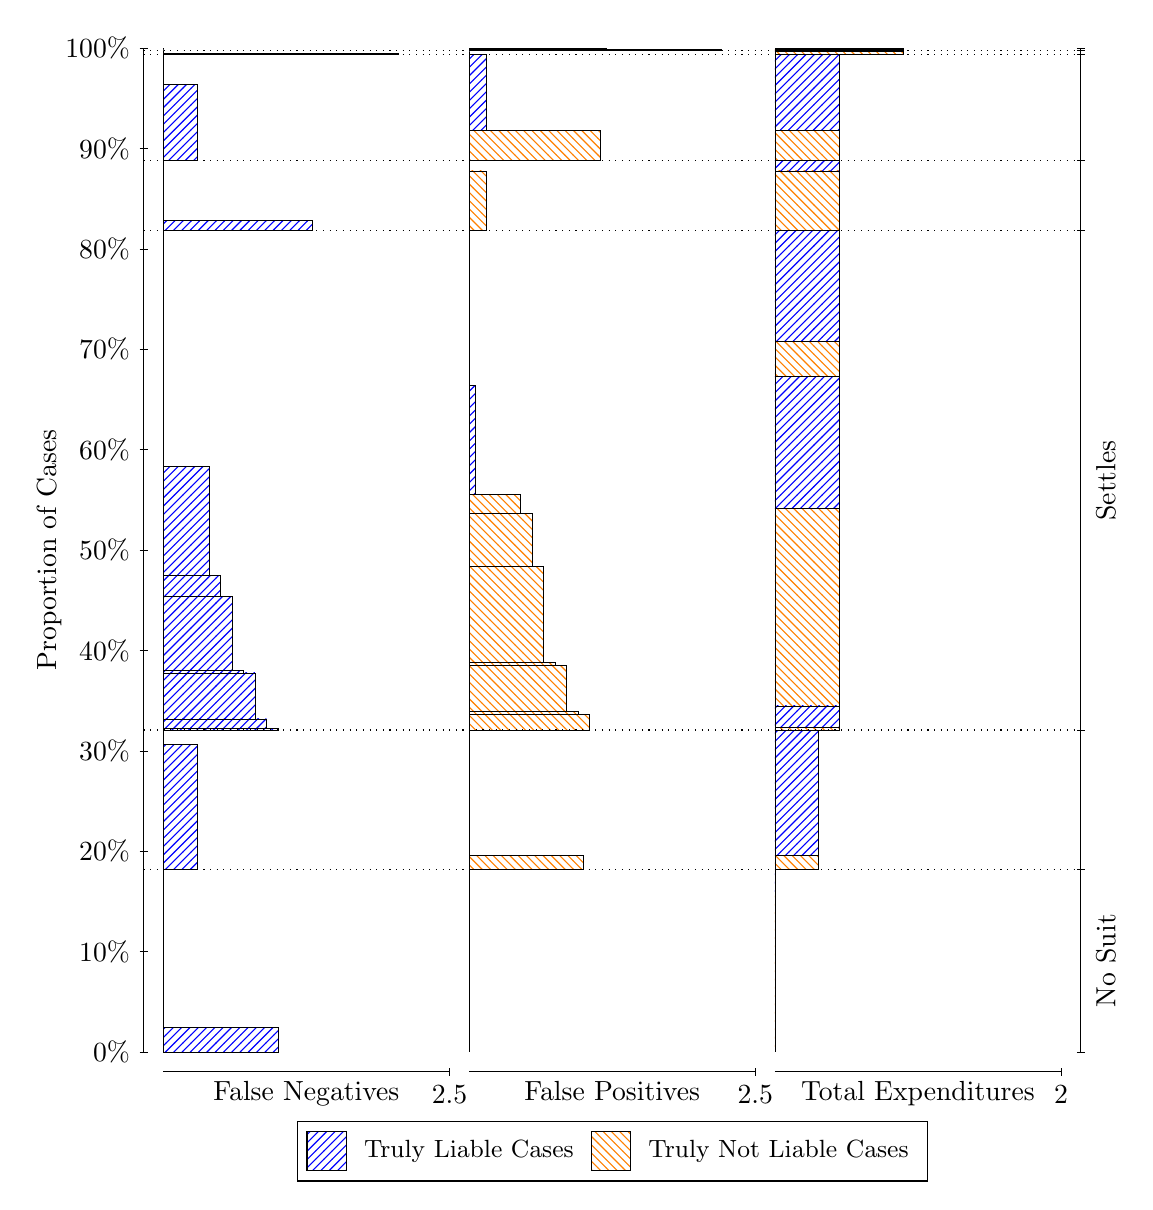
\begin{tikzpicture}
\draw[black, very thin] (1.5,1.75) -- (1.5,14.5);
\node[rotate=90, text=black, anchor=center] at (0.3, 8.125) {Proportion of Cases};
\draw[black, very thin] (1.45,1.75) -- (1.55,1.75);
\node[text=black, anchor=east] at (1.45, 1.75) {0\%};
\draw[black, very thin] (1.45,3.025) -- (1.55,3.025);
\node[text=black, anchor=east] at (1.45, 3.025) {10\%};
\draw[black, very thin] (1.45,4.3) -- (1.55,4.3);
\node[text=black, anchor=east] at (1.45, 4.3) {20\%};
\draw[black, very thin] (1.45,5.575) -- (1.55,5.575);
\node[text=black, anchor=east] at (1.45, 5.575) {30\%};
\draw[black, very thin] (1.45,6.85) -- (1.55,6.85);
\node[text=black, anchor=east] at (1.45, 6.85) {40\%};
\draw[black, very thin] (1.45,8.125) -- (1.55,8.125);
\node[text=black, anchor=east] at (1.45, 8.125) {50\%};
\draw[black, very thin] (1.45,9.4) -- (1.55,9.4);
\node[text=black, anchor=east] at (1.45, 9.4) {60\%};
\draw[black, very thin] (1.45,10.675) -- (1.55,10.675);
\node[text=black, anchor=east] at (1.45, 10.675) {70\%};
\draw[black, very thin] (1.45,11.95) -- (1.55,11.95);
\node[text=black, anchor=east] at (1.45, 11.95) {80\%};
\draw[black, very thin] (1.45,13.225) -- (1.55,13.225);
\node[text=black, anchor=east] at (1.45, 13.225) {90\%};
\draw[black, very thin] (1.45,14.5) -- (1.55,14.5);
\node[text=black, anchor=east] at (1.45, 14.5) {100\%};

\draw[black, very thin] (13.4,1.75) -- (13.4,14.5);
\draw[black, very thin] (13.35,1.75) -- (13.45,1.75);
\node[anchor=west] at (13.35, 1.75) {};
\draw[black, very thin] (13.35,4.0678) -- (13.45,4.0678);
\node[anchor=west] at (13.35, 4.0678) {};
\draw[black, very thin] (13.35,5.8384) -- (13.45,5.8384);
\node[anchor=west] at (13.35, 5.8384) {};
\draw[black, very thin] (13.35,12.18) -- (13.45,12.18);
\node[anchor=west] at (13.35, 12.18) {};
\draw[black, very thin] (13.35,13.072) -- (13.45,13.072);
\node[anchor=west] at (13.35, 13.072) {};
\draw[black, very thin] (13.35,14.421) -- (13.45,14.421);
\node[anchor=west] at (13.35, 14.421) {};
\draw[black, very thin] (13.35,14.471) -- (13.45,14.471);
\node[anchor=west] at (13.35, 14.471) {};
\draw[black, very thin] (13.35,14.5) -- (13.45,14.5);
\node[anchor=west] at (13.35, 14.5) {};

\draw[black, very thin, pattern color=blue, pattern=north east lines] (1.75,1.75) rectangle (3.2033,2.0615);
\draw[black, very thin, pattern color=orange, pattern=north west lines] (1.75,2.0615) rectangle (1.75,4.0678);
\draw[black, very thin, pattern color=blue, pattern=north east lines] (1.75,4.0678) rectangle (2.186,5.6555);
\draw[black, very thin, pattern color=orange, pattern=north west lines] (1.75,5.6555) rectangle (1.75,5.8384);
\draw[black, very thin, pattern color=blue, pattern=north east lines] (1.75,5.8384) rectangle (3.2033,5.8592);
\draw[black, very thin, pattern color=blue, pattern=north east lines] (1.75,5.8592) rectangle (3.058,5.9799);
\draw[black, very thin, pattern color=blue, pattern=north east lines] (1.75,5.9799) rectangle (2.9127,6.5633);
\draw[black, very thin, pattern color=blue, pattern=north east lines] (1.75,6.5633) rectangle (2.7673,6.5993);
\draw[black, very thin, pattern color=blue, pattern=north east lines] (1.75,6.5993) rectangle (2.622,7.5317);
\draw[black, very thin, pattern color=blue, pattern=north east lines] (1.75,7.5317) rectangle (2.4767,7.8004);
\draw[black, very thin, pattern color=blue, pattern=north east lines] (1.75,7.8004) rectangle (2.3313,9.1836);
\draw[black, very thin, pattern color=orange, pattern=north west lines] (1.75,9.1836) rectangle (1.75,12.18);
\draw[black, very thin, pattern color=blue, pattern=north east lines] (1.75,12.18) rectangle (3.6393,12.312);
\draw[black, very thin, pattern color=orange, pattern=north west lines] (1.75,12.312) rectangle (1.75,13.072);
\draw[black, very thin, pattern color=blue, pattern=north east lines] (1.75,13.072) rectangle (2.186,14.04);
\draw[black, very thin, pattern color=orange, pattern=north west lines] (1.75,14.04) rectangle (1.75,14.421);
\draw[black, very thin, pattern color=blue, pattern=north east lines] (1.75,14.421) rectangle (4.7293,14.434);
\draw[black, very thin, pattern color=orange, pattern=north west lines] (1.75,14.434) rectangle (1.75,14.471);
\draw[black, very thin, pattern color=orange, pattern=north west lines] (1.75,14.471) rectangle (1.75,14.484);
\draw[black, very thin, pattern color=blue, pattern=north east lines] (1.75,14.484) rectangle (1.75,14.5);
\draw[black, very thin, pattern color=orange, pattern=north west lines] (5.6333,1.75) rectangle (5.6333,3.7564);
\draw[black, very thin, pattern color=blue, pattern=north east lines] (5.6333,3.7564) rectangle (5.6333,4.0678);
\draw[black, very thin, pattern color=orange, pattern=north west lines] (5.6333,4.0678) rectangle (7.0867,4.2507);
\draw[black, very thin, pattern color=blue, pattern=north east lines] (5.6333,4.2507) rectangle (5.6333,5.8384);
\draw[black, very thin, pattern color=orange, pattern=north west lines] (5.6333,5.8384) rectangle (7.1593,6.0361);
\draw[black, very thin, pattern color=orange, pattern=north west lines] (5.6333,6.0361) rectangle (7.014,6.0738);
\draw[black, very thin, pattern color=orange, pattern=north west lines] (5.6333,6.0738) rectangle (6.8687,6.6572);
\draw[black, very thin, pattern color=orange, pattern=north west lines] (5.6333,6.6572) rectangle (6.7233,6.7019);
\draw[black, very thin, pattern color=orange, pattern=north west lines] (5.6333,6.7019) rectangle (6.578,7.9212);
\draw[black, very thin, pattern color=orange, pattern=north west lines] (5.6333,7.9212) rectangle (6.4327,8.5868);
\draw[black, very thin, pattern color=orange, pattern=north west lines] (5.6333,8.5868) rectangle (6.2873,8.8345);
\draw[black, very thin, pattern color=blue, pattern=north east lines] (5.6333,8.8345) rectangle (5.706,10.218);
\draw[black, very thin, pattern color=blue, pattern=north east lines] (5.6333,10.218) rectangle (5.6333,12.18);
\draw[black, very thin, pattern color=orange, pattern=north west lines] (5.6333,12.18) rectangle (5.8513,12.939);
\draw[black, very thin, pattern color=blue, pattern=north east lines] (5.6333,12.939) rectangle (5.6333,13.072);
\draw[black, very thin, pattern color=orange, pattern=north west lines] (5.6333,13.072) rectangle (7.3047,13.453);
\draw[black, very thin, pattern color=blue, pattern=north east lines] (5.6333,13.453) rectangle (5.8513,14.421);
\draw[black, very thin, pattern color=orange, pattern=north west lines] (5.6333,14.421) rectangle (5.6333,14.457);
\draw[black, very thin, pattern color=blue, pattern=north east lines] (5.6333,14.457) rectangle (5.6333,14.471);
\draw[black, very thin, pattern color=orange, pattern=north west lines] (5.6333,14.471) rectangle (8.8307,14.484);
\draw[black, very thin, pattern color=blue, pattern=north east lines] (5.6333,14.484) rectangle (7.3773,14.5);
\draw[black, very thin, pattern color=orange, pattern=north west lines] (9.5167,1.75) rectangle (9.5167,3.7564);
\draw[black, very thin, pattern color=blue, pattern=north east lines] (9.5167,3.7564) rectangle (9.5167,4.0678);
\draw[black, very thin, pattern color=orange, pattern=north west lines] (9.5167,4.0678) rectangle (10.062,4.2507);
\draw[black, very thin, pattern color=blue, pattern=north east lines] (9.5167,4.2507) rectangle (10.062,5.8384);
\draw[black, very thin, pattern color=orange, pattern=north west lines] (9.5167,5.8384) rectangle (10.334,5.8761);
\draw[black, very thin, pattern color=blue, pattern=north east lines] (9.5167,5.8761) rectangle (10.334,6.1449);
\draw[black, very thin, pattern color=orange, pattern=north west lines] (9.5167,6.1449) rectangle (10.334,8.6578);
\draw[black, very thin, pattern color=blue, pattern=north east lines] (9.5167,8.6578) rectangle (10.334,10.33);
\draw[black, very thin, pattern color=orange, pattern=north west lines] (9.5167,10.33) rectangle (10.334,10.776);
\draw[black, very thin, pattern color=blue, pattern=north east lines] (9.5167,10.776) rectangle (10.334,12.18);
\draw[black, very thin, pattern color=orange, pattern=north west lines] (9.5167,12.18) rectangle (10.334,12.939);
\draw[black, very thin, pattern color=blue, pattern=north east lines] (9.5167,12.939) rectangle (10.334,13.072);
\draw[black, very thin, pattern color=orange, pattern=north west lines] (9.5167,13.072) rectangle (10.334,13.453);
\draw[black, very thin, pattern color=blue, pattern=north east lines] (9.5167,13.453) rectangle (10.334,14.421);
\draw[black, very thin, pattern color=orange, pattern=north west lines] (9.5167,14.421) rectangle (11.152,14.457);
\draw[black, very thin, pattern color=blue, pattern=north east lines] (9.5167,14.457) rectangle (11.152,14.471);
\draw[black, very thin, pattern color=orange, pattern=north west lines] (9.5167,14.471) rectangle (11.152,14.484);
\draw[black, very thin, pattern color=blue, pattern=north east lines] (9.5167,14.484) rectangle (11.152,14.5);
\draw[black, dotted] (1.5,4.0678) -- (13.4,4.0678);
\draw[black, dotted] (1.5,5.8384) -- (13.4,5.8384);
\draw[black, dotted] (1.5,12.18) -- (13.4,12.18);
\draw[black, dotted] (1.5,13.072) -- (13.4,13.072);
\draw[black, dotted] (1.5,14.421) -- (13.4,14.421);
\draw[black, dotted] (1.5,14.471) -- (13.4,14.471);
\draw[black, very thin] (1.75,1.5) -- (5.3833,1.5);
\node[text=black, anchor=north] at (3.5667, 1.5) {False Negatives};
\draw[black, very thin] (5.3833,1.45) -- (5.3833,1.55);
\node[text=black, anchor=north] at (5.3833, 1.45) {2.5};

\draw[black, very thin] (5.6333,1.5) -- (9.2667,1.5);
\node[text=black, anchor=north] at (7.45, 1.5) {False Positives};
\draw[black, very thin] (9.2667,1.45) -- (9.2667,1.55);
\node[text=black, anchor=north] at (9.2667, 1.45) {2.5};

\draw[black, very thin] (9.5167,1.5) -- (13.15,1.5);
\node[text=black, anchor=north] at (11.333, 1.5) {Total Expenditures};
\draw[black, very thin] (13.15,1.45) -- (13.15,1.55);
\node[text=black, anchor=north] at (13.15, 1.45) {2};

\node[text=black, centered, rotate=90] at (13.72, 2.9089) {No Suit};

\node[text=black, centered, rotate=90] at (13.72, 9.0091) {Settles};





\draw (7.449999999999999,1.5) node[draw=none] (baseCoordinate) {};
\begin{scope}[align=center]
        \matrix[scale=0.5, draw=black, below=0.5cm of baseCoordinate, nodes={draw}, column sep=0.1cm]{
            \node[rectangle, draw, minimum width=0.5cm, minimum height=0.5cm, pattern color=blue, pattern=north east lines] {}; &
            \node[draw=none, font=\small, text=black] (B) {Truly Liable Cases}; &
            \node[rectangle, draw, minimum width=0.5cm, minimum height=0.5cm, pattern color=orange, pattern=north west lines] {}; &
            \node[draw=none, font=\small, text=black] (B) {Truly Not Liable Cases}; \\
            };
\end{scope}

\end{tikzpicture}
\end{document}